\documentclass{report}
\usepackage[english]{babel}
\usepackage{microtype}
\usepackage{amsmath,amssymb}
\usepackage{amsthm}
\usepackage[round]{natbib}
\usepackage[all]{xy}
\usepackage{graphicx}
\usepackage{enumerate}
\usepackage{qtree}
\usepackage{mdframed}
\usepackage{tikz-dependency}
\bibliographystyle{plainnat}
\author{}
\title{}
\newtheoremstyle{indented}{8pt}{8pt}{\addtolength{\leftskip}{2.5em}}{}{\bfseries}{.}{.5em}{}
\theoremstyle{indented}
\newtheorem{metric}{Metric}
\newtheorem{notion}{Notion}

\begin{document}
\maketitle
\tableofcontents

\chapter{Introduction}

Ever since ..., many have been inspired by this quote of Warren Weaver, one of the very first researchers to aim for the construction of systems automatically performing translation task.:

\begin{quote}
\textit{When I look at an article in Russian, I say: `This is really written in English, but it has been coded in some strange symbols. I will now proceed to decode.}
\end{quote}

Evidently, automatic translation is not as easily solved as Weaver thought at the time. Over 60 years later, we still have no systems that automatically produce translations with a quality comparable to that of a human translator (anders). The field of Machine Translation has grown much bigger, currently there are (something that indicates the size of the field of Machine Translation), and may different methods have been investigated. This work focuses on one such method: compositional translation.\\
%Explain what compositional translation is (based on compositionality of language, mapping between the grammars generating them. Describe principle of compositionality of translation
In many fields in which translations occur (computer science, logic, philosophy), computational translation is a very common method. The semantics of an expression in a certain logic, for instance, can be unambiguously determined by considering the terms and the methods used to combine them. Translating such an expression into another logical language can be effectively carried out by translating these terms and methods into the terms and methods particular for the second logic. For natural language, compositional translation is not as straight forward.
%words have multiple meanings, sentences are vague and ambiguous, building blocks are unclear blabla
Not only do we have to deal with problems as disambiguation and context, we also do not dispose a set of rules uniquely generating our language. In fact, many have argued against language as a completely compositional system (ref). Examples of arguments against compositionality.\\
I guess a short section about the formal strength of compositionality.


% although not every grammar is suitable for compositional meaning assignment, the class of languages that can be analyzed is not restricted, nor are the meanings that can be assigned: any recursively enumerable language can be generated by a compositional grammar, and any semantics can be dealt with in a compositional way. 
%Is this helpful? Is NL recursively enumerable? What about ambiguity

However, none of this teaches us if compositional translation is a reasonable strategy for translating natural language. Intuitively, it seems reasonable that 'who-did-what-to-whom-relations' are universal for languages, but exploiting this fact in translation has proven to be a non-trivial task. The present work does not aim to develop a model for compositional translation of language, but rather attempts to empirically analyse if it is realistic to aim for one.\\
%Explain how this question becomes practical
Although this question is of theoretical nature, blabla explain that we have to deal with data such that it merely transforms to the question: can we find compositionality in the corpora we are training on, that an be of use in translation models. We will therefore also pay some attention to the use of the results, and make suggestions for future work.

\section*{Related Work}

This is not the first work concerned with the ... phenomena related to compositionality

\cite{fox2002phrasal} investigated if syntactic phrases tend to stay together during translation from French to English.
%Explain how this has to do with compositionality
%Explain how she did this
%Mention issue of phrasal translation
%Discuss her results

Even more directly related to this work is the empirical study presented by \cite{hwa2002evaluating}. \citeauthor{hwa2002evaluating} empirically evaluate the \textit{Direct correspondence assumption (DCA)}, the assumption that for two sentences that are each others translation, the syntactic relations in one sentence directly map to the syntactic relations in the other. %Explain similarity with compositionality of translation principle
%Explain that Hwa argues that the DCA cannot account for some well known and fundamental linguistic facts
%Explain that this is also what they show
%Explain what she does after (making linguistic adaptations)
%Discuss these result: problem with building blocks, still doesn't show that ocmpositional translation isn't possible.. (what else?)


\section*{Thesis Setup}

%Rewrite this when the rest is written
As mentioned before, the primary goal of this thesis is to investigate whether predicate-argument relations are preserved during translation. To do so, a tree will be searched that respects both the alignment (completely) and as much of the predicate-argument relations present in the source sentence as possible. The resulting tree will be scored according to how many of the predicate argument relations were allowed by the alignment, thus yielding a compositionality measure for the sentence.\\
The following chapter will give some theoretical background: it will explain the notion of alignment-respecting trees (anders) and provide some information on the grammar formalism used to extract predicate-argument relations.\\
Chapter \ref{chapter:impl} give more information on the implementation of the research, while the actual experiments and their results will be presented in chapter \ref{chapter:exp}.
%We probably also need a section about compositionality (lets see how that is gonna fit in)
%Describe the rest


\chapter{Background}

Make a nice introductory statement to this chapter. Provide theoretical background, the field in which this research is conducted blabla.


\section{(Statistical) (Machine) Translation}
%Maybe I can write this section really in the light of compositionality
%Some background description of SMT, do I need this, what for?
A short section that gives some information about the field this research is conducted in, and helps to see the relevance of this work on a larger scale
% Explain how Machine Translation started
% Explain how we went from word based to phrase based to rule based?
% Explain the current status of the use of compositionality in translation?




\section{Compositional Translation}

The method of compositional translation is based on the idea that sentences that are each others translation do not only have the same meaning, but have also a similar semantic structure. 

%Explain assumptions: language is compositional, translations are literal..

which captures the intuition that translation should preserve the meaning, but also the form, as far as possible. For example, it accounts for the fact that \textit{all ravens are black} is an adequate translation of the Dutch \textit{alle raven zijn zwart} and that the logical equivalent sentence \textit{if something is not black it is not a raven} is not an adequate translation. \cite{landsbergen1989power}


%Explain that there are examples in which this is not the case: idomatic expressions in which there is no direct relation between form and meaning, syntactic mismatch, example hwa
%--> solution: making strong rules and bigger basic expressions
%problem with transformational capacity of idioms

%for more examples, refer to landsbergen

%Landsbergen also gives an example for which no compositional solution is found (cross the river swimming), explain that this is a theoretical problem rather than a practical one. Solution is not elegant, but a grammar automatically derived from a parallel corpus won't be elegant anyways :p

%Furthermore, it assumes that language is compositional (of course), maybe explain a bit more about this, perhaps give some of examples from \cite{janssen1996compositionality} explain that these are mostly discourse like problems, which is a separate part from machine translation --> generate ALL linguistically accepted translations

\begin{quote}
The meaning of an expression is a function of the meaning of its parts and syntactic rule by which they are combined. \cite{partee1984compositionality}
\end{quote}


%I feel like somewhere I also need to say that translation is a relation between languages in this framework and that the grammars therefore need to be isomorphic (i.e. basic expressions and rules need to have translation-equivalents in the other language)

\section{Translation Structures?}

%Investigation of compositionality: see if we can find compositional structures. Explain the restrictions that compositionality puts on these structures, and how these can be seen/found in data
We will define this set of structures.

\subsection{Alignments}

%Dit moet anders, maar weet nog even niet hoe, in Khalil paper staat ook een definitie zie ik nu.
An alignment is a mapping between the words of a sentence in one language, and the words in its translation in another. Given a source sentence $s = s_0 \ldots s_n$ and its translation $t = t_0 \ldots t_m$, an alignment $a$ is a set of pairs $(x,y)$ with $x\in \{0,1,\ldots,n\}$ and $y\in \{0,1,\ldots,m\}$ that describes which source position is translated to which target position. Words can align to several words on the other side, as well as none, which yields different types of alignments. A one to one alignment is an alignment in which no word or source or target side is aligned to more than one word, in a many-to-one alignment target words may have links to more than one source side position. The alignment in Figure \ref{fig:alignment} is a one-to-many alignment, as the word 'likes' is aligned to both 'houdt' and 'van', but no target position that has more than one link. (anders) The least restrictive kind of alignment is the many-to-many alignment, in which both source and target words may have multiple alignment links. An alignment in which the source and target words are in the same order is called a monotonic alignment.

\begin{figure}[!ht]
\centering
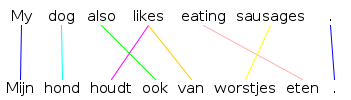
\includegraphics[scale=0.6]{alignment.png}
\caption{An alignment of the English sentence `My dog also likes eating sausages.' and its translation `Mijn hond houdt ook van worstjes eten'.%schrijf welke tool is gebruikt
}\label{fig:alignment}
\end{figure}

Naturally, a mapping from source to target words is not given for a translation\footnote{Even for humans it turns out to be a not so trivial task to find them, maybe ref naar manual corpus}, and devising algorithms to find them is one of the problems in Machine Translation (anders).
%Say that there are many approaches but that the IBM tools are still most commonly used
%Describe IBM alignments: they are a by-product of the word-based IBM models but only many-to-one alignments --> run in both positions and take union, intersection or use other heuristics to obtain alignment
%Tell that there are some manual corpora available (+references?)
%Maybe examples of problems in alignments

\subsection{Phrase Pairs}

% Describe that the links that describe which source words are translated into which target words also give us information about how larger units are possibly translated into each other (related to the compositionality principle)

%The first ones to define this? I don't know I keep running into this reference when people are talking about phrases \cite{och2004alignment}


The phrases consistent with the alignment are thus phrases whose translation is also a phrase. Note that in this context the word `phrase' denotes any arbitrary sequence of words that is contiguous, and it not restricted to linguistic phrases. For instance, the phrases consistent with the alignment in Figure \ref{fig:alignment} (the dot aside) are: ([0,0], [1,1], [2,3], [4,4], [5,5], [0,1], [2,3], [4,5], [1,3], [0,4], [2,5], [0,5]). In which [x,y] includes all words from position $x$ to position $y$. Note that the word 'like' does not form a phrase on its own, as it translates into two non-adjacent words in the Dutch target sentence.\\
The number of phrases in an alignment is dependent on the type of alignment (anders).
%Explain that monotonic alignments do not restrict at all, and a completely monotonic alignment thus has many phrases: \frac{n\times n+1}{2}

%Tell about algorithm for extracting tight phrase pairs efficiently??

\subsection{Alignment Trees}

%Explain that on an even larger scale the alignment and phrase pairs also tell us how the whole sentence was possibly composed compositionally. This compositional structure can be represented as a tree, in which the nodes are phrases consistent with the alignment.
%Example of an alignment tree for 2.1

\begin{figure}
\Tree [.[0,6] [.[0,1] [.[0,0] my ] [.[1,1] dog ] ] [.[2,6] [.[2,4] [.[2,2] also ] [.[3,3] likes ] [.[4,4] eating ] ] [.[5,6] [.[5,5] eating ] [.[6,6] sausage ] ] ] ] ]
\caption{A possible alignment tree for the alignment of Figure \ref{fig:alignment}}
\end{figure}

% Say something that compares to fox, explain that it is a weaker condition in a sense, because things like 'ne pas' do not necessarily cause crossings
%Explain interest of such trees to MT (studying recursive properties, reordering, rule based systems)
% Link to literature about this topic, explanation of literature (I think I need to find references in Khalils 


%Say that every alignment can be assigned at least one compositional structure this way (although it might be a structure that is completely flat), and is therefore less strict than the definition of fox. Often many structures can be assigned. Maybe iets zeggen over hoeveel, en iets over empirische analyse Khalil en Gideon.

%\subsection{Hierarchical Alignment Trees}\label{sec:hats}

\section{Dependency Grammar}

%Introduction: maybe some history about dependency grammars and how they came about (refer to phrase structure grammars)

%Explain why dependency relations seems suitable for the task at hand: we want to see if predicate argument relations stay intact, dependencies are predicate argument relations
%Maybe also some arguments from other studies that support the suitability of dependency grammars (higher cohesion dependency grammars fox e.g, work quirk & menezes.

%Describe stanford dependency representation

The Stanford Dependency representation distinguishes five different styles. As an elaborate description of these styles, as well as an extensive list of the relations in all of them, can be found in the Stanford typed dependency manual \citep{de2008stanford}, in this thesis just a short summary will be given.
\paragraph{Basic Dependencies} The basic dependency style contains, as the name suggests, all the basic dependencies present in the sentence. A basic dependency structure is a fully connected projective dependency structure, that is, there are no crossing dependencies.
\paragraph{Collapsed dependencies} In the collapsed representation several dependencies involving function words are collapsed to get direct dependencies between content words. Furthermore, additional dependencies that break the tree structure are considered, which means the resulting dependency graph is not guaranteed to be acyclic or even a tree. There exist another 2 variants of the collapsed dependency representation, one in which conjunct dependencies are propagated, and one in which the dependencies that do not preserve the tree structure are omitted.
\paragraph{Non-collapsed dependencies} The last representation gives the basic dependencies as well as the extra ones which break the tree structure.

%Describe available parsers.
Zeg iets over de beschikbare parsers \cite{de2006generating}
%Probeer misschien nog wat andere literatuur te vinden over dependency grammar

\section{The Best Tree}

Describe that we need a way to decide how good a tree is and that there are different ways to do that. Present evaluation metrics.

\subsection{Shared Notation}

Firstly, we will present some notation that is shared along the different metrics.

\begin{notion}
$T_d$ will refer to a dependency tree of a sentence $s = w_1 \dots w_n$, formed by a set of dependencies $D = \{ (i,j) |$ there is a dependency arrow from word $w_i$ to word $w_j \}$.
\end{notion}

\begin{notion}
If $T_d$ is a dependency tree for $s$, $w$ is a word in $s$ and $i$ and $j$ are the maximum and minimum positions, respectively, that can be reached from $w$ by following the directed dependency arrows. Then span($w$) = $[i,j]$.
\end{notion}

\begin{notion}
$T_a$ will be used to refer to an alignment tree of a sentence $s = w_1 \dots w_n$. The label $i-j$ will refer to the node that dominates span $[i,j]$. The highest node of $T_a$ will be denoted with $N_{T_a}$
\end{notion}

\begin{notion}
Let $T_d$ be a dependency tree with dependencies $D$, Then $D' = \{ (i,\textrm{span}(j))$ $|$ $D(i,j) \land 1 \leq i,j \leq n \}$ is the set in which each dependent is replaced by its span.
\end{notion}

\begin{notion}
If $N$ is a node in a tree $T_a$, $C_N$ denotes the set of child constituents of this node. If node $N$ dominates words $i$ to $j$ in $s$, then $dom(N)= [i,j]$
\end{notion}

\subsection{Metric 1}

A dependency tree $T_d$ tells us exactly of which are the smaller parts of the sentence and how they are combined to obtain the complete sentence. Consider for instance the dependency tree of the sentence "My dog also likes eating sausage" (Figure \ref{fig:deptree1}).

\begin{figure}[!h]\label{fig:deptree1}
\centering
\begin{dependency}[theme=simple]%[hide label]
\begin{deptext}[column sep=.5cm, row sep=.1ex]
%PRP\$ \& NN \& RB \&[.5cm] VBZ \& VBG \& NN \\
My \& dog \& also \& likes \& eating \& sausage \\
\end{deptext}
\deproot{4}{}
\depedge{2}{1}{poss}
\depedge{4}{2}{nsubj}
\depedge{4}{3}{xvmod}
\depedge{4}{5}{xcomp}
\depedge{5}{6}{dobj}
\end{dependency}
\caption{Stanford Dependency Tree}
\end{figure}

\noindent The dependency tree tells us that 'likes' is the head word of the sentence, and that the sentences is composed of 4 parts: the head 'likes', its modifier 'also', its noun subject whose head is 'dog' and the open clausal complement whose head is 'eating'. The complement and subject are further divisible in, 'My' and 'dog', and 'eating' and 'sausage', respectively. Intuitively, for every relation in the dependency parse, we can check whether this relation exists in an alignment tree $T_a$, by checking if the word and its depending subtrees are siblings in $T_a$. The evaluation metric used in this first experiment is based upon this intuition.

\begin{metric}\label{m1}
Let $s = w_1 w_2 \dots w_n$ be a sentence, and $T_d$ and $T_a$ its dependency tree and an alignment tree, respectively. The score of $T_a$ is defined as the score of its highest node $N_{a}$:

$$
E(N_a,D) = \sum_{c\in C_{N_a}} E(c,D)+ \sum_{c_1\in C_{N_a}} \sum_{c_2\in C_{N_a}} B(c_1,c_2)
$$

\noindent With base case $E(N,D) = 0$ and $B(c_1,c_2) = 1$ iff  $(c_1,c_2)\in D'$. Dividing the resulting score by $|D'|$ will result in a normalized score.
\end{metric}

\noindent  Note if this definition is strictly followed more than half of the sibling checks is redundant, an algorithm computing the score of a tree would not have to perform them all.

\subsection{Metric 2}

Explain that metric 1 reflects the similarity with the dependency parse, rather than giving a reasonable measure of compositionality. Explain why this is, that a part of the score can trivially be reached by just making a flat tree. Explain how to fix this. Explain that evaluation metric 2 won't alter the ordering of the trees, just their scores.
Explain that metric 2 thus just differs in the set of relations it considers: instead of considering all relations from the dependency parse, it only considers the relations that reflect compositionality, which captures the intuition that completely flat trees should be assigned a 0 score. Note that this means that this therefore does not alter the ranking of the trees set by metric 1, it just alters the scores associated with the trees.

\begin{metric}\label{m2}
Let $s = w_1 w_2 \dots w_n$ be a sentence, and $T_d$ and $T_a$ its dependency tree and an alignment tree, respectively. The score of $T_a$ is defined as the score of its highest node $N_{a}$:

$$
E(N_a,D) = \sum_{c\in C_{N_a}} E(c,D)+ \sum_{c_1\in C_{N_a}} \sum_{c_2\in C_{N_a}} B(c_1,c_2)
$$

\noindent With base case $E(N,D) = 0$ and $B(c_1,c_2) = 1$ iff  $|dom(c_2)| > 1 \land (c_1,c_2)\in D'$ the part of the sentence covered by $c_2$. Dividing the resulting score by $|D'|$ will result in a normalized score.
\end{metric}

Note that normalizing the score will sometimes result in zero division for shorter sentences whose dependency parses display no compositional structure, in this cases we will define the score of the sentence to be 0.

%CHAPTER DESCRIBING THE IMPLEMENTATION OF THE EXPERIMENTS

\chapter{Implementation}
\label{chapter:impl}
%Alternative title: compositionality in practice
Describe that recursive alignment trees are very useful for investigating the recursive properties of translation. Describe empirical research \cite{simaan2013hats}.\\
Describe that in this work we will use the structures for investigating the preservation of predicate argument structures, as extracted from dependency parses. Explain that we let go of the restriction that the HATs should be minimally branching (+reason), say something about that we only look at the tree structure and not at the reordering, as this is for the theoretical question unimportant.
Unaligned words also all considered. Say that this significantly increases the complexity of the task, but that this is less of a problem as the purpose is analysis, thus we only have to do it once.



\section{Setup}

Explain that the main framework scores an alignment according to a given set of preferred relations between nodes that are siblings in the tree, or nodes that are mother and child. Explain that it is designed to be easily extendible for testing different properties of the tree.

Explain that tests were conducted with different evaluation metrics, information about which can be found in the description of the experiments.

%Do not know what level of detail is required here...
Briefly discuss how: for each alignment a grammar is created that uniquely generates all Recursive Alignment Trees. The different productions of this grammar are assigned a score proportional to the preferred number of mother child relations that it generates. (similar to a probability, but not the same). A parser is used to find the optimal alignment tree (i.e. the alignment tree with the highest number of preferred mother child relations), and its score.
%Maybe say something about the scoring and how different things can be tested but that one needs to think about scores for the productions


\section{Implementation}

Open source implementation that consists of different parts

\begin{itemize}
\item the part that deals with the dependency relations, extracts different relations from them and assigns labels to spans
\item part that generates the context free grammars, details about this is implemented? graph approach, spans found by an algorithm similar to Zhangs.. def of phrases is slightly different, an emtpy node can also be a phrase.
\item parser, external viterbi parser from nltk toolkit \citep{bird2009natural}, slightly adapted such that it can dael with scores that are not probabilities 
\end{itemize}

The only thing that is thus required is an evaluation metric

\chapter{Empirical}

\section{Datasets}

Tell something about datasets, preparation, blabla
%Denk dat ik dit toch net iets anders wil doen, zodat ik alle resultaten in 1 tabel kan zetten enzo

\section{Experiments}

Describe which experiments were done (with which datasets, which metrics..)

\section{Results}

\begin{table}\label{tab:scores}
\begin{tabular}{llll}
Experiment 1 & metric 1 & dataset 1 & 0.84\\
Experiment 2 & metric 2 & dataset 1 & 0.52\\
Experiment 3 & metric 2 & dataset 2 & 0.79\\
\end{tabular}
\caption{Average sentence score of corpus (vul in) according to different metrics.}
\end{table}


The average sentence score of this corpus is 0.830827979565.

\section{Discussion}

Discussion of the results of the experiments, analysis of the results

At the first sight, the results of experiment 1 seem very promising: on average over 80\% of the dependency relations are supported by the alignment. However, the trees in the outputted corpus seems strikingly flat, even for long sentences. Although one could argue that this is also compositional in some aspect, it is definitely not the kind of compositionality that is interesting in the light of Machine Translation. The obtained score might have reflected the similarity with the dependency parses well, but seems no good measure for compositionality. This is mainly caused by the fact that not all relations in the dependency parse actually reflect compositionality. The average fraction of relations that express word to word relations over the entire corpus is 0.56 %(this is not just over the 46 sentences parsed, fix that!)
, which means that a score of 0.56 could be obtained by simply assigning every sentence in the corpus a completely flat tree. Experiment 2 addresses this problem, altering the evaluation metric such that the score of an alignment tree primarily reflects compsitionality, rather than similarity with the dependency tree of the sentence.


\subsection{Analysis}

There are 4 main reasons that could result in a low score for evaluation metric 2:
\begin{enumerate}
\item Errors in the translation or non literal translation;
\item Errors in the alignment;
\item Error in the dependency parse;
\item The sentence cannot be compositionally translated.
\end{enumerate}

For X scored sentences a tree with a score higher than 0.70 was found. Manual analysis of the other 46-X analysed sentences (\ref{tab:class} showed that most of the low compositionality scores weren't for lack of possible compositional translations, but were merely due to translation errors, errors in sentence alignment and for the larger part errors in the alignment.

\begin{table}[!h]\label{tab:class}
\begin{tabular}{|l|l|}
\hline
Translation Error & \\
Alignment Error & \\
Parse Error &\\
No Compositional translation possible & \\
\hline
\end{tabular}
\caption{Manual analysis of the X scored}
\end{table}

If the lack of compositionality found in the corpus was really caused by poor automatic alignments, one would expect the score of a corpus scored manually to be higher. This hypothesis is tested in experiment 3.

Een stuk hoger indeed, analysis of de bomen lager dan 0.7 in deze dataset

Wat zijn mogelijke opties voor extensie?

\chapter{Discussion and Future Work}

short summary of findings and what they mean

future work: source reordering, treebank to learn translation structure


\chapter{Conclusion}

%THINGS I SHOULDN'T FORGET TO MENTION!

% zeg iets over dat we op deze manier nicely omgaan met phrasal translations

% put statistics about the data, the dependency parses, everything

% ook wat analyses over complexiteit e.d. max grootte van de grammatica's dat soort zaken

% niet zo tevreden over hoe dependency grammars met conjunction omgaan, collapsed dependencies doen dit wel beter trouwens, misschien moet ik daar nog eens naar kijken. Collapsed dependencies doen soms ook al wat werk met idiom (zie tabel 3)

%Maybe moet ik nog iets zeggen over dat compositionaliteit aangenomen wordt in veel systemen (e.g. rule-based systemen)

%Geen enkel vertaalsysteem vertaalt een zin 'in zijn geheel', altijd in stukken

% Bouw iets in in dat dependency programma dat oneindige recursie tegengaat

% Bouw meer checks in die kijken of de input wel consistent is

\bibliography{thesisDH}

\end{document}
